\begin{figure}[h]
  \centering
  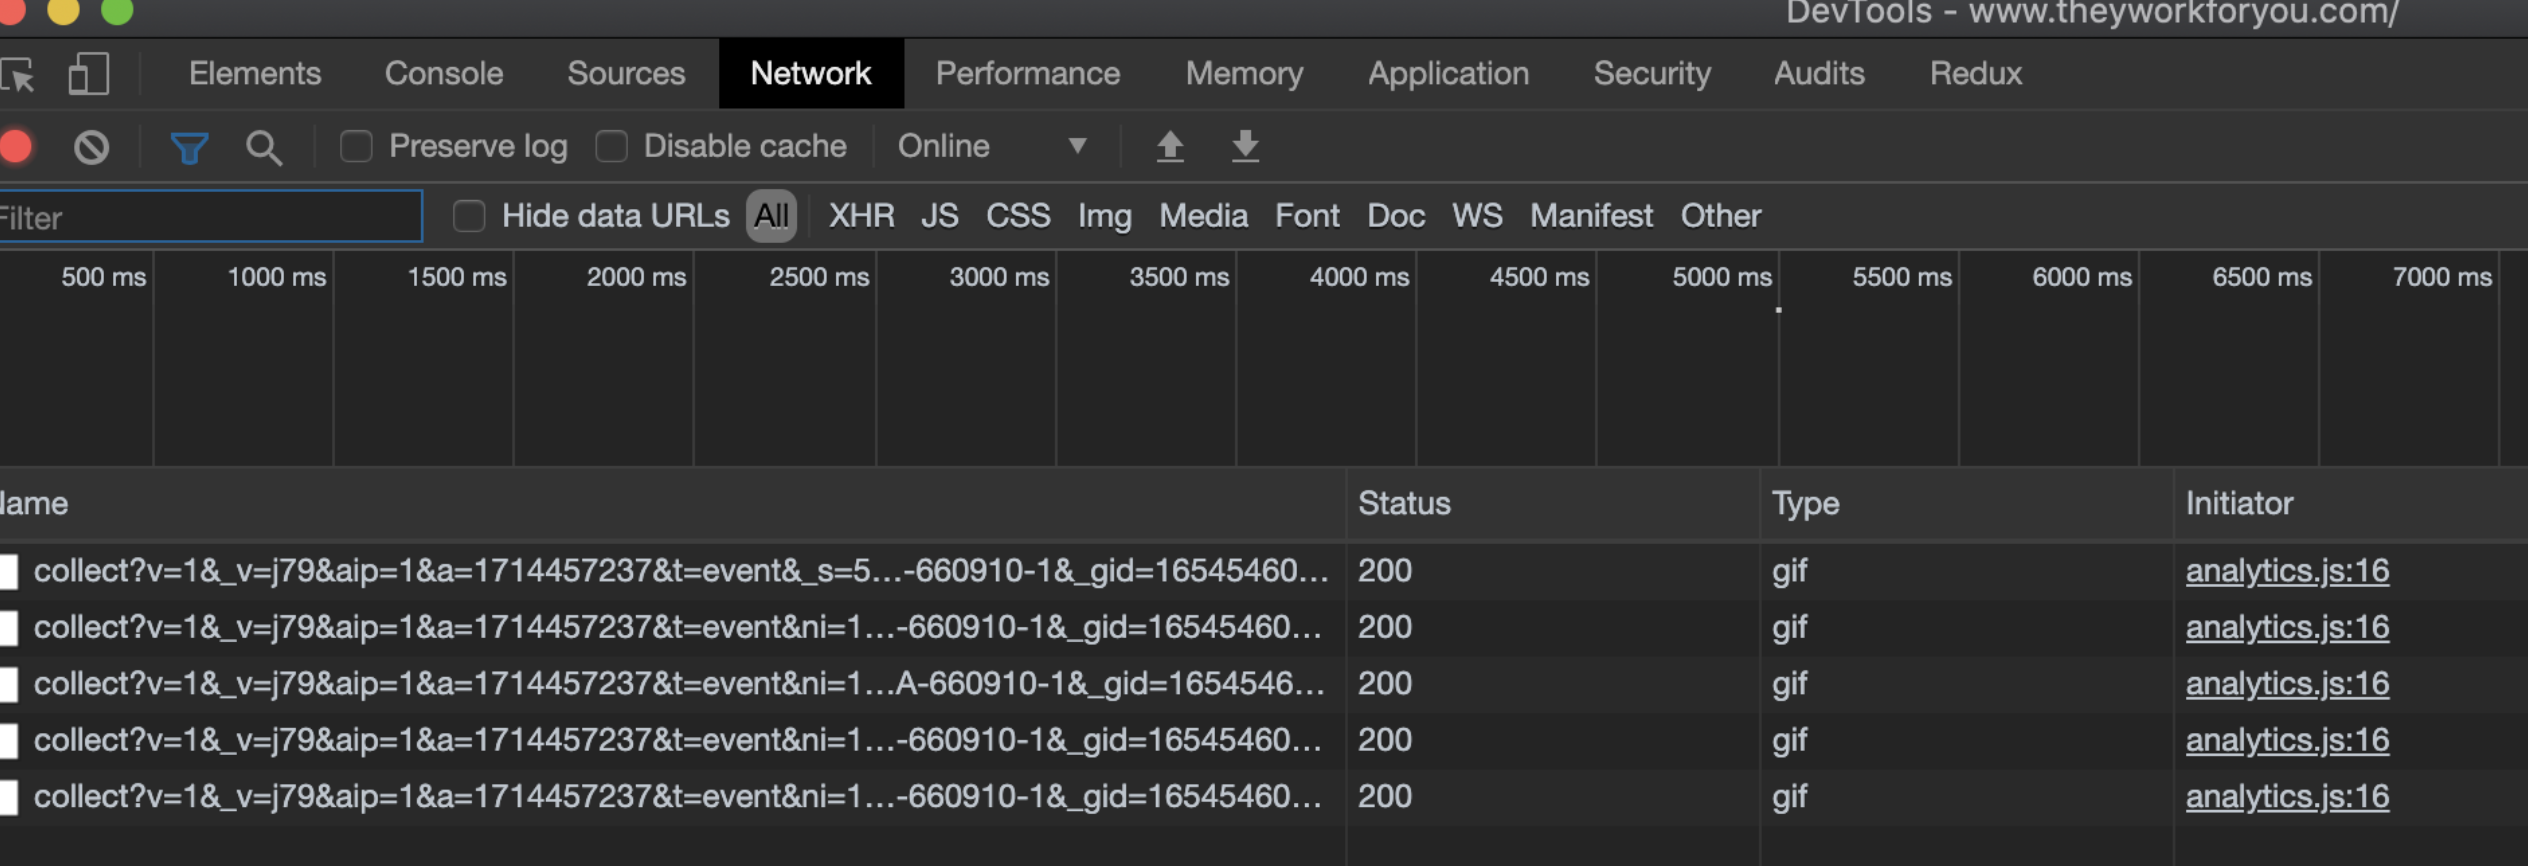
\includegraphics[scale=0.25]{images/they-work-for-you-challenges-google-analytics}
  \caption{They Work for You: Google analytics}
  \label{fig:they-work-for-you-challenges-google-analytics}
\end{figure}

Figure \ref{fig:they-work-for-you-challenges-google-analytics} depicts a screen shot of network traffic generated by the They Work for You site when viewed using the Chrome browser.
The five entries towards the bottom of the screenshot show that the site is sending information about user activity to Google Analytics \cite{google-analytics} on an approximately second by second basis.
That is, the client browser that that the author of this essay used to view the site is sending information to Google Analytics.
This finding suggests that They Work For You as an organisation do have access to statistics about user activity on their site.
However, given that They Work for You is a small charitable organisation, it may well be the case that make use of the free version of Google Analytics.
If that is the case, then the rights to the aggregated analytics data are held by Google, and that may explain why they don’t publish data about usage of the site.